% This is LLNCS.DOC the documentation file of
% the LaTeX2e class from Springer-Verlag
% for Lecture Notes in Computer Science, version 2.4
\documentclass{llncs}
\usepackage{llncsdoc}
\usepackage[hyphens]{url}
\usepackage[pdftex]{graphicx}     
\usepackage{float}
\usepackage{tablefootnote}
\usepackage{hyperref}

\hyphenation{block-chain}
\hyphenation{block-chains}
\hyphenation{Block-chain}
\hyphenation{Block-chains}

	%%%%%%%%%%%%%%%%%%%%%%%
	%% Added to enable numbering for subsubsections, otherwise they would look like paragraphs which is ugly
	%%%%%%%%%%%%%%%%%%%%%%%
	
	\makeatletter
	\renewcommand\subsubsection{\@startsection{subsubsection}{3}{\z@}%
		{-18\p@ \@plus -4\p@ \@minus -4\p@}%
		{0.5em \@plus 0.22em \@minus 0.1em}%
		{\normalfont\normalsize\bfseries\boldmath}}
	\makeatother
	\setcounter{secnumdepth}{3}

%
\begin{document}


	{
	%
	\title{Tezos-based Vehicular Ad Hoc Blockchains\\ - \\ \small Vision Paper - Version 0.5\\\small \today}
	
	\author{Benjamin Leiding \and William V. Vorobev}
	
	\institute{ 
		Chorus Mobility\\
		Email: hello@chorus.mobi\\
	}
	
	\maketitle

	%% ----------------------------------------------------------------
	%% ----------------------------------------------------------------

	\begin{abstract}

		% A good abstract:
		%1.) What is the paper about?
		%2.) What is the SoA?
		%3.) What is the detected gap?
		%4.) What are the main questions to be answered pertaining to the gap?
		%5.) Why is the solution good/better than other solutions?

		The next generation of tightly interconnected vehicles offers a variety of new technologies as well as business opportunities. Vehicles form so-called vehicular ad hoc networks (VANETs). Sophisticated systems of interconnected cars in the context of VANETs assume a full coverage of 5G networks to unfold their full potential. However, nowadays network infrastructure is neither 5G-ready nor does it provide reliable and full coverage of all areas that might be relevant for VANET-based networks. Hence, the conventional mode of operations of all nodes being connected to one blockchain at all times is not feasible. In addition, traditional blockchains also require every node to process each transaction and smart contract commands which are highly inefficient. Therefore, we present a solution based on so-called mobile ad hoc blockchains that enable groups of nodes involved in any kind of collaboration to effectively form temporary networks and coordinate themselves. 

		Another critical requirement of VANETs and interconnected vehicles is security. The safety of network participants does not only depend on the vehicle's hardware, but also on the correctness of the software that controls the interaction and transaction within the network. Formal verification is a common way to address the issue proving the correctness of software. The self-amending blockchain Tezos supports Turing-complete smart contracts and also offers built-in formal verification of their programming languages, thereby fostering the security of our solution.

		This whitepaper fills the gap by introducing Vehicular Ad Hoc Tezos Blockchains based on mobile ad hoc blockchains that allow groups of nodes to be temporarily disconnected from the overall network but still being able to enact and transact on a local network level for the duration of their interaction. We present the advantages of the system, outline the requirements and goals, as well as the architecture of the system.



	\end{abstract}
	
	
	\keywords{VANET, Formal Verification, Tezos, Mobile Ad Hoc Blockchains, Blockchain, Smart Contracts, Interoperability, Vehicle Networks, V2X}

	%% ----------------------------------------------------------------
	%% ----------------------------------------------------------------
	
	\section{Introduction}
		\label{s:introduction}

		Despite steadily growing public transport networks and systems, especially in most first world countries, cars are still the default standard for urban transportation. In the US, ``about 86 percent of all workers commuted to work by private vehicle, either driving alone or carpooling" \cite{mckenzie2015drives}, even though in recent years the numbers remained relatively stable after decades of consistent increase. Similar applies to other industrial countries \cite{netherlandsPublicTransport}\cite{zealand2006car} though the overall percentage of vehicle commuters in Europe is lower than in the US \cite{commuteUSvsEurope}. While it was normal for the last few decades to own a vehicle and commute on a day-by-day basis, the future will be radically different due to the progressing evolution of self-driving cars and autonomous vehicles. The car-sharing economy that developed in recent years in combination with autonomous cars results in a so called \textit{passenger economy} \cite{intelPassengerEconomy}. Users no longer own cars, instead just hop on an autonomous car, pick a destination and get delivered without any human interaction. An Intel report estimates the size of this economy to be around US\$ seven trillion in 2050 \cite{intelPassengerEconomy}.

		A key technology for the next generation of tightly interconnected vehicles are so-called vehicular ad-hoc networks (VANETs) \cite{bibid}. Vehicles form VANETs enable vehicle-to-vehicle (V2V), vehicle-to-infrastructure (V2I), vehicle-to-human (V2H), or in general vehicle-to-everything (V2X) communication and interaction. In our previous research paper \cite{our-own-paper}\cite{something-for-V2whatever}\cite{bibid}, we presented a blockchain-based system that enables a manufacturer agnostic platform solution that allows VANET participants to enact and transact any kind of services and goods. Sophisticated networks of interconnected cars require full coverage of 5G networks to unfold their full potential \cite{bibid}. However, nowadays network infrastructure is neither 5G-ready nor does it provide reliable and full coverage of all areas that might be relevant for VANET-based networks. Hence, the conventional mode of operations of all nodes being connected to one blockchain at all times is not feasible \cite{bibid}. In addition, traditional blockchains such as Bitcoin \cite{nakamoto_bitcoin:2008} and Ethereum \cite{wood2014ethereum} also require every node to process each transaction and smart contract commands which are highly inefficient. Therefore, we present a solution based on so-called mobile ad hoc blockchains that enable groups of nodes involved in any kind of collaboration to effectively form temporary networks and coordinate themselves. They only connect to nodes they need to be connected to, depending on the context, for the duration of their interaction.
		
		Another critical requirement of VANETs and interconnected vehicles is security. The safety of network participants does not only depend on the vehicle's hardware, but also on the correctness of the software that controls the interaction and transaction within the network. Formal verification is a common way to address the issue proving the correctness of software with respect to a certain formal specification or property using formal methods of mathematics \cite{bibid}\cite{bibid}. The self-amending blockchain platform Tezos \cite{tezosWhitepaper} does not only support Turing complete smart contracts, it also offers built-in formal verification of their smart contract programming languages, thereby fostering the security of our solution.



%%%%%%%%%%%%%%%%%%%%%%%%%%%%%%%%%%%%%%%%%%%%%%%%%%%%%%%%%%%%%%%%%%%%%%

%		RQ: How to ?
%		RQ-1: What is the corresponding architecture of the Vehicular Ad Hoc Tezos Blockchain?
%		RQ-2: What are the detailed network and communication processes?
%		RQ-3: What kind of use cases and application scenarios exist?


%%%%%%%%%%%%%%%%%%%%%%%%%%%%%%%%%%%%%%%%%%%%%%%%%%%%%%%%%%%%%%%%%%%%%%
		
		This work fills the gap by introducing a Tezos-based vehicular ad hoc blockchain solution, thereby answering the question of how to enable vehicular ad hoc blockchains that allow groups of nodes to be temporarily disconnected from the overall network but still being able to enact and transact on a local network level for the duration of their interaction? In order to answer this question with a separation of concerns, we pose the following sub-questions: What is the corresponding architecture of the Vehicular Ad Hoc Tezos Blockchain? What are the detailed network and communication processes? What kind of use cases and application scenarios exist?
		
		The remainder of this paper is structured as follows: Section~\ref{s:section-2} introduces supplementary literature and related work. Section~\ref{s:section-3} outlines the system architecture our solution. Afterwards, Section~\ref{s:section-4} expands on the network communication processes, followed by Section~\ref{s:section-5} that introduces example use cases and application scenarios. Finally, Section~\ref{s:section-6} concludes this work and provides an outlook on future work.


	%% ----------------------------------------------------------------
	%% ----------------------------------------------------------------

	\section{Technical Background and Supplementary Literature}	
		\label{s:section-2}
		
		The following section provides background information and describes related works regarding previous ideas and concepts that focus on a blockchain-based VANET platforms. First, Section~\ref{ss:blockchain-intro} introduces the general concepts of blockchain technology, terms and frameworks. Afterwards, Section~\ref{ss:vanets} and Section~\ref{ss:formal-verification} focus on the fundamentals of vehicular ad-hoc networks as well as formal verification. Finally, Section~\ref{ss:related-work} introduces related work. 
					
		%% ----------------------------------------------------------------
		%% ----------------------------------------------------------------	
		
		\subsection{Blockchain Technology}
			\label{ss:blockchain-intro}
			
			As the name suggests, a blockchain consists of a chronologically ordered chain of blocks. Every block consists of a certain number of validated transactions and each of those block links to its predecessor by a hash reference. As a result, changing the content of one block also changes all succeeding blocks and hence breaks the chain. All blocks are stored on and verified by all participating nodes. While the initial Bitcoin blockchain only supported a very limited set of scripting instructions, the next generation of blockchain platforms, e.g., Ethereum \cite{wood2014ethereum}, Qtum \cite{qtumWhitepaper}, or Tezos \cite{tezosWhitepaper}, provide Turing-complete programming languages on the protocol-layer level in order to enable smart contract capabilities. Smart contracts are ``orchestration- and choreography protocols that facilitate, verify and enact with computing means a negotiated agreement between consenting parties" \cite{qtumWhitepaper}. Hence, the entities participating in the enactment of a smart contract establish binding agreements and deploy applications using such smart contracts in order to provide blockchain-based applications. Those application are as versatile as smart contracts itself and enable services including the finance sector \cite{nguyen2016blockchain}\cite{saltWhitepaper}, academic and business authentication and identity solutions \cite{leidingUnchained}\cite{CivicWhitepaper}\cite{AuthcoinLeiding2016MCIS}\cite{mccorry2015authenticated}\cite{SelfkeyWhitepaper}, reputation systems \cite{SemadaWhitepaper} as well as platforms for Internet-of-Things (IoT) applications \cite{christidis2016blockchains}\cite{ouaddah2017towards}. 	
			
			The blockchain concept is particularly interesting for the V2X economy for three reasons. First, it removes the need for trusted third parties and instead enables trust-less transaction enactment. Second, transactions that were agreed up on cannot be changed later on since the underlying blockchain is tamperproof. Third, no human interaction is required for any kind of transaction between vehicles or machines in general.


		%% ----------------------------------------------------------------
		%% ----------------------------------------------------------------	
		
		\subsection{Vehicular Ad-Hoc Networks - VANETs}
			\label{ss:vanets}

			Communication between vehicles, road infrastructure and Internet-based services is a key enabler for the upcoming generation of vehicles. So called vehicular ad-hoc networks provide an abstract concept that models the different components that are required for V2V, V2I, or V2X communication. Figure \ref{fig:vanets} illustrates the main components of VANETs: Vehicles, on-board-units (OBUs), application-units (AUs) and road-side-units (RSUs).\\
			RSUs are placed  along the road side or in dedicated locations such as at crossroads. Typically, RSUs provide short range communication based on IEEE 802.11p radio technology but can also be equipped with other network devices in order to provide communication within the infrastructural network \cite{al2014comprehensive}. OBUs are mounted onto a vehicle and used for data exchange. To do so, short range wireless- or radio communication is used to exchange these information \cite{baldessari2007car}. Closely linked to the OBU is the AU, they might even reside in the same physical unit or as a mobile until that is regularly removed from the vehicle (e.g smartphones). The AU provides an execution environment for applications that utilize the OBU's communication capabilities \cite{al2014comprehensive}\cite{baldessari2007car}.\\	
			\begin{figure}[ht]
				\centering
				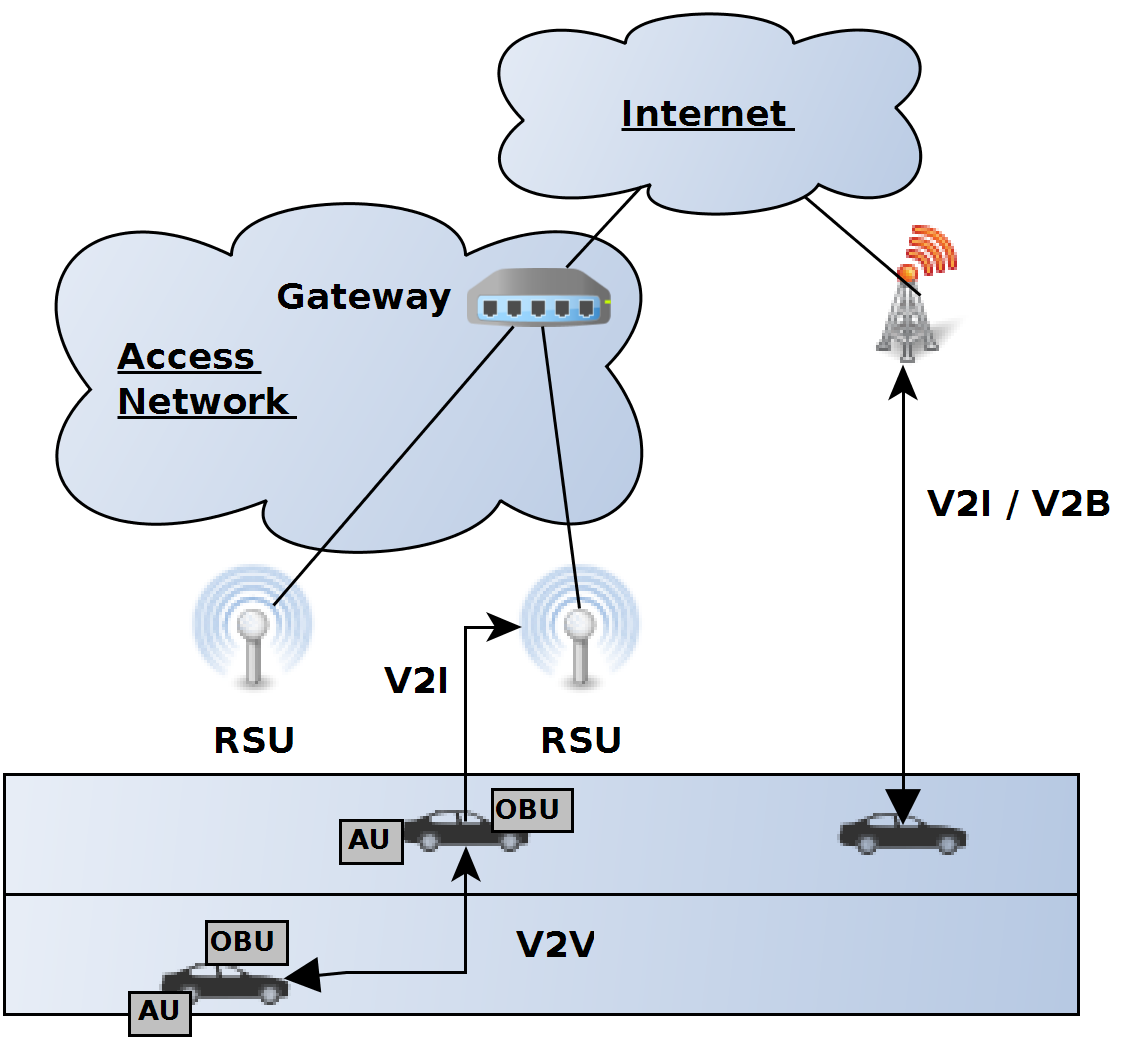
\includegraphics[scale=0.2]{Figures/Vanets.png}
				\caption{General VANET architecture (Based on \protect\cite{baldessari2007car} and \cite{leiding2016self})}
				\label{fig:vanets}
			\end{figure}			
			Communication in VANETs occurs either inside a vehicle between AUs and OBU, wirelessly between different vehicles (V2V), vehicles and infrastructure (V2I) or vehicles and the infrastructure via broadband (V2B) \cite{faezipour2012progress}. For authentication purposes, each network participant is equipped with a unique public/private key pair that resides in a tamper-proof-device (TPD). In blockchain terms, the TPD is similar to an external hardware wallet.

		%% ----------------------------------------------------------------
		%% ----------------------------------------------------------------	
		
		\subsection{Formal Verification}
			\label{ss:formal-verification}

			Another critical requirement of VANETs and interconnected vehicles is security. The safety of network participants does not only depend on the vehicle's hardware, but also on the correctness of the software that controls the interaction and transaction within the network. Formal verification is a common way to address the issue proving the correctness of software according to a specification using formal methods of mathematics. ``A formal method is a mathematically-based technique used in computer science to describe properties of hardware and/or software systems. It provides a framework within which large complex systems may be specified, developed, and verified in a systematic rather than ad-hoc manner. A method is formal if it has a sound mathematical basis, typically given by a formal specification language" \cite{wing1990specifier}. The concept of formal verification is not new at all and over many decades, several approaches and concepts for formal methods have been introduced, e.g., Statecharts \cite{harel1987statecharts}, abstract state machines (ASMs) \cite{gurevich1995evolving}, Petri nets \cite{petri1962kommunikation}, the Calculus of Communicating Systems \cite{milner1989communication} and $\pi$-calculus \cite{milner1992calculus}, as well as timed automata \cite{alur1994theory} and communicating sequential processes \cite{hoare1978communicating}.
						
			The self-amending blockchain platform Tezos\footnote{\url{https://tezos.com/}} \cite{tezosWhitepaper} does not only support Turing complete smart contracts, it also offers built-in formal verification of their smart contract programming languages. The idea is to leverage the built-in formal verification mechanism to ensure a correct behavior of the involved smart contracts, thereby enhancing the security of applications within VANETs. Especially due to the progressing digitalization and inter-connection of vehicles, the dependencies of large and complex software to operate those vehicles and networks grows tremendously and hence becomes more vulnerable to unintended security use cause by badly written code.s

			
		%% ----------------------------------------------------------------
		%% ----------------------------------------------------------------	
		
		\subsection{Related Work}
			\label{ss:related-work}

			In our previous work \cite{chorusWhitepaper}\cite{chorus2018MCIS}, we introduced a blockchain-based value transaction layer protocol for vehicular ad hoc networks that is supposed to fuel vehicle economy. However, previous work focused on providing a protocol layer and an abstract platform architecture whereas this work extends our previous efforts and suggests a specific Tezos-based implementation.

			MONET \cite{monetWhitepaper} introduced the idea mobile ad hoc blockchains in combination with the Babble consensus algorithm. The downside of Babble is that it is based on Hashgraph \cite{hashgraphWhitepaper} which is patented in the U.S. and requires a license which limits widespread adoption of their solution. In addition, MONET relies on Ethereum and its smart contracting languages which do not offer built-in formal verification as Tezos does. Finally, the authors do mention a public/private key based identity solution that is necessary for their permissioned blockchain. However, how to prevent sybil node attacks and ensure a mapping between identity and its owner is still unclear.

			Cosmos \cite{cosmosWhitepaper} proposed a network architecture of independent and parallel blockchains that rely on the Tendermint consensus protocol - a partially synchronous BFT consensus protocol derived from the DLS consensus algorithm \cite{dwork1988consensus}. They also introduce the concept of an inter-blockchain communication (IBC) protocol that allows for interaction among the parallel blockchains.
			
		%% ----------------------------------------------------------------
		%% ----------------------------------------------------------------	
		

	%% ----------------------------------------------------------------
	%% ----------------------------------------------------------------

	\section{System Design and Architecture}
		\label{s:section-3}
		
		%RQ-1: What is the corresponding architecture of the Vehicular Ad Hoc Tezos Blockchain?
		
		As previously mentioned in Section~\ref{ss:related-work} the concept of mobile ad hoc blockchains is not new and has been recently applied to mobile ad hoc networks (MANETs) in the form of the MONET project \cite{monetWhitepaper}. The following sections now outline the process of adapting the general concept of mobile ad hoc blockchains to VANETs. VANETs are a sub-category of MANETs. There are two main differences between the two types of networks. First, not all entities in VANETs are mobile and only sparsely connected to the Internet, e.g., RSU and infrastructure components. They are stationary and hence it easy to establish permanent Internet access for them, making them the perfect relay stations. Second, in VANETs the communication nodes are moving on predefined roads in contrast to nodes in MANETs that are not bound to any restrictions. Note that this definition excludes flying vehicles such as drones from VANETs in the context of this work.  
		
		Section~\ref{ss:architecture-overview} presents the high-level architecture of the VANET blockchain, followed by Section~\ref{ss:identities} that discusses the topics of identities within our system. Finally, Section~\ref{ss:consensus} outlines the consensus strategies for vehicular ad hoc blockchains.
		
		%% ----------------------------------------------------------------
		%% ----------------------------------------------------------------	
		
		\subsection{System Architecture}
			\label{ss:architecture-overview}
			
			The system architecture illustrated in Figure~\ref{fig:architecture-overview} extends the commonly used VANET concept of Figure~\ref{fig:vanets} that we introduced earlier. RSUs, vehicles equipped with OBUs and AUs as well as the infrastructure backend remain the same. However, similar to the concept of MONET, mobile nodes, i.e., vehicles, can form so called mobile ad hoc blockchains. Only vehicles within a certain range of each other form such networks. To do so, they agree up on an initial list of participants, while new nodes may join later or current nodes leave - depending on the context.		
			\begin{figure}[H]
				\centering
				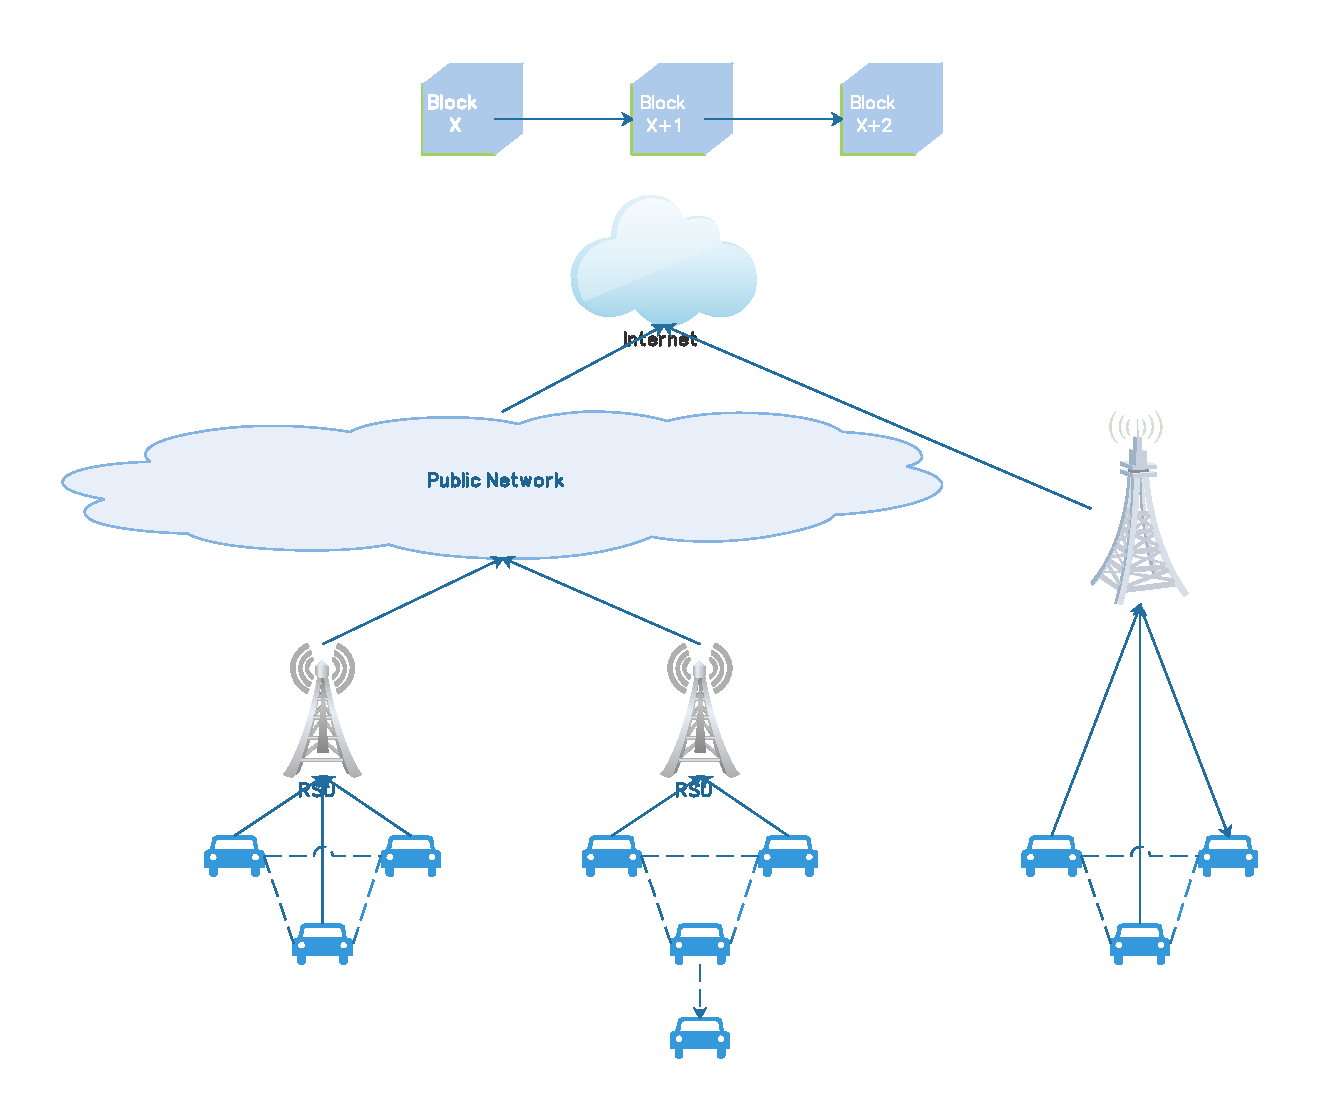
\includegraphics[scale=0.5]{Figures/20180904_monet-vanet.pdf}
				\caption{Caption.}
				\label{fig:architecture-overview}
			\end{figure}
			Nodes that form a vehicular ad hoc blockchain agree up on transactions on their own (see Section~\ref{ss:consensus} for more details on consensus) and periodically forward state and status information to RSUs or other infrastructure entities. Those permanent and fixed components have a direct connection to the Internet as well as the VANET backend which enables them to relay received information from the specific independent vehicular ad hoc blockchains to the main blockchain (depicted at the top of Figure~\ref{fig:architecture-overview}). Vehicular ad hoc blockchains are either directly connected to RSUs or to some other kind of infrastructure that providers access to the Internet. Vehicles that do not have access to a RSU or alternative options can use a mesh-based approach where they connected to an ad hoc network that relays their information to the destination (middle of Figure~\ref{fig:architecture-overview}). Due to the missing full network coverage along the existing road infrastructure, there might be periods where a complete set of nodes is only interconnected among each others, but not to the main network. Our system tolerates such temporary disconnects assuming that a mesh-based Internet connection can be established within a few hops.

		%% ----------------------------------------------------------------
		%% ----------------------------------------------------------------	
		
		\subsection{Tezos Hubs and Ad Hoc Blockchains}
			\label{ss:blockchain-hubs}
			
			Besides the temporary vehicular ad hoc blockchains, we also envision - similarly to  \cite{monetWhitepaper}, \cite{cosmosWhitepaper} and \cite{chorus2018MCIS}- a set of Tezos hubs that act as master blockchain for our network. This could be the Tezos main network or an alternative independently operated Tezos chain - as long as they ensure permanent availability and Internet connection. All network participants are to create their own hub or deploy any other solution to support their applications. The Tezos hubs are operated by validators and rely on Proof-of-Stake to reach consensus. The intention of the hub structure is to enable permanent availability of network supporting services that enable inter-blockchain communication (see Section~\ref{ss:inter-blockchain-communication}), identity services (see Section~\ref{ss:identities}), or backend services for applications of the vehicular ad hoc blockchains.
			
		%% ----------------------------------------------------------------
		%% ----------------------------------------------------------------	

		\subsection{Identities}
			\label{ss:identities}
		
			Tamper-proof-devices (TPDs) are a standard component of VANETs. They usually contain a public/private key (similar to wallet addresses) pair that uniquely identifies a vehicle and serves for authentication and signing as well as verification purposes. Usually, TPDs are pre-equipped by the car manufacturer and built into the vehicle's hardware. In the context of blockchains, an identity is further required in most consensus algorithms to uniquely identify participants. Moreover, a mapping between public/private keys (that constitute an identity) and vehicles is also necessary to prevent sybil node attacks. 
			%rephrase - from securecomm paper
			This type of attack is a common issue in large-scale peer-to-peer (P2P) systems, where hostile or faulty computing elements threaten the security of the whole network. Single faulty entities may be able to present multiple identities, thereby controlling a substantial fraction of the system, consequently undermining its functionality and security \cite{douceur2002sybil}.	
			%rephrase end			
			Unfortunately, the majority of current cars does not have a such a TPD that could constitute a cars identity. Hence, an alternative solution is required. We are currently evaluating different approaches. First, equipping vehicles on our own with small hardware devices that can easily be attached to vehicles and contain a TPD that ensures an identity binding. Second, utilizing smartphones as identity providers. Third, using blockchain-based validation and authentication protocols such as Authcoin  \cite{leiding2017securing}\cite{AuthcoinLeiding2016MCIS}\cite{leiding2017mapping}.
		
		%% ----------------------------------------------------------------
		%% ----------------------------------------------------------------	

		\subsection{Blockchain Consensus in VANETs}
			\label{ss:consensus}
			
			In the context of blockchains, consensus algorithms are usually used to agree on a set of transactions that constitutes the next block that is added to the chain. Proof-of-Work \cite{nakamoto_bitcoin:2008} and Proof-of-Stake \cite{bibid} are most common and used for example by Bitcoin and Ethereum. For both major consensus algorithms, different flavors exists as well as a large variety of alternative protocols. However, almost all current state of the art algorithms suffer some kind of disadvantage, e.g., scalability issues, security issues, efficiency issues, and so on \cite{bibid}\cite{bibid}. Figure~\ref{fig:bft-scalability} illustrates a collection of consensus algorithms and their scalability as well as performance properties. 
			\begin{figure}
				\centering
				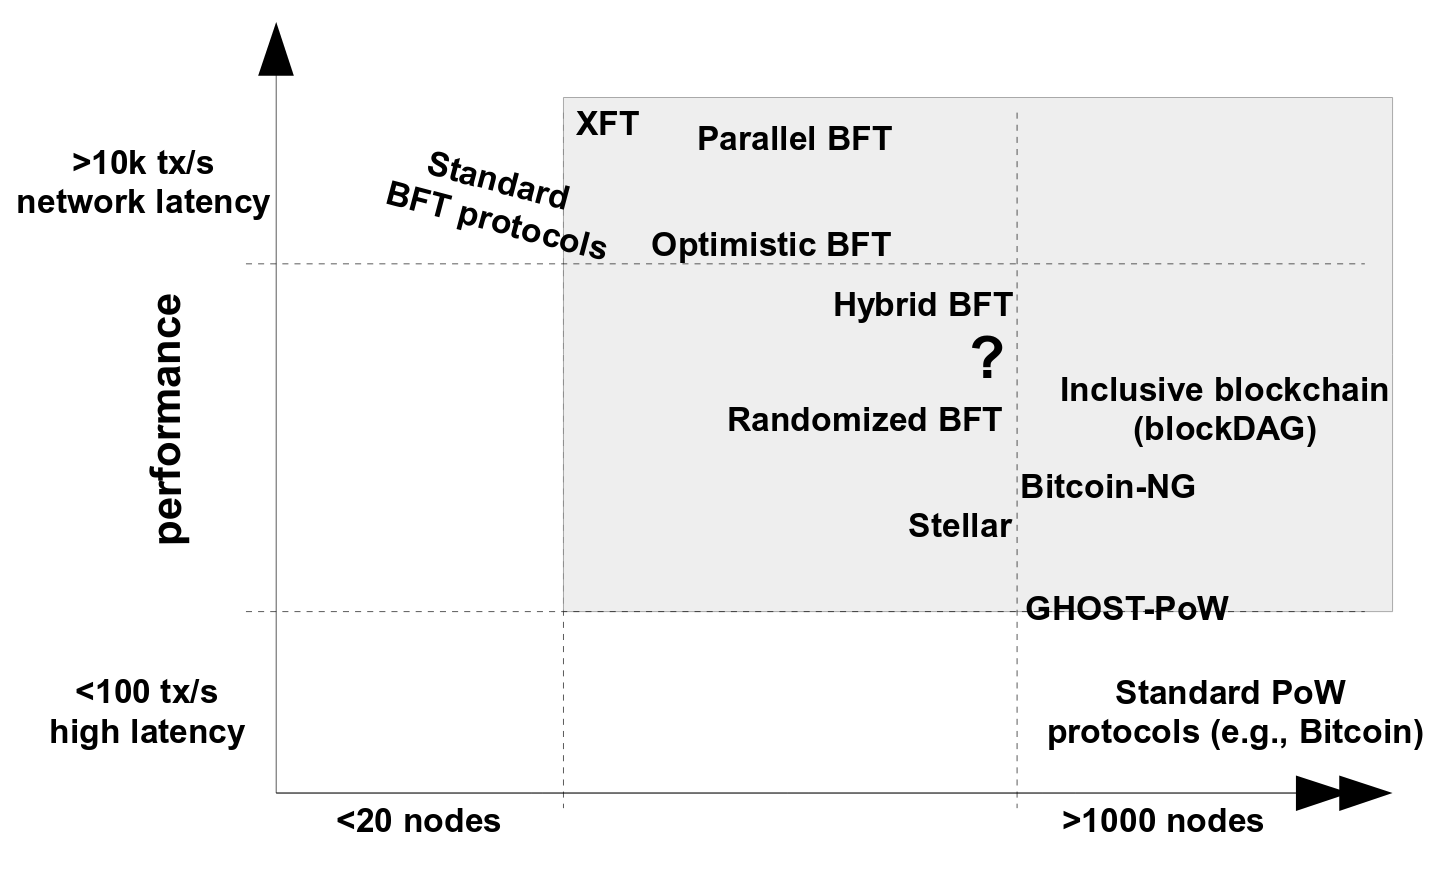
\includegraphics[scale=0.25]{Figures/BFT/20180904_BFT-scalability.png}
				\caption{Caption (Source: \cite{vukolic2015quest}).}
				\label{fig:bft-scalability}
			\end{figure}
			Those problems become even more complex in the  context of mobile- and vehicular ad hoc blockchains due to the large number disjunct chains that exist in parallel as well as the the fact that entities are sometimes only connected in a mesh network without connection to the Internet which makes consensus on a global level even more difficult. In this context, timing assumptions become important. Consensus protocols might be fully synchronous which means that all messages are delivered within a pre-defined time  $x$ whereas asynchronous consensus protocols only ensure that all messages are eventually delivered \cite{bibid}. Between those two extrema different sub-categories such as eventually synchronous, partial synchronous and weakly synchronous consensus algorithms exist \cite{bibid}\cite{bibid}\cite{bibid}. In vehicular ad hoc blockchains a fully asynchronous consensus protocol is  desirable due to the sparse connectivity of nodes and missing connection guarantees among nodes.
						
			There are different protocols that aim to offer solutions in this regard. The Babble consensus algorithm \cite{bibid} relies on a leaderless, asynchronous, Byzantine fault tolerant (BFT) algorithm that is based on Hashgraph \cite{hashgraphWhitepaper}.However, Hashgraph is patent protect in the U.S. and therefore limited in us. Alternative protocols such as \cite{miller2016honey}, \cite{bibid} and \cite{bibid} exist besides Hashgraph with certain limitations. We are currently researching different solutions that enable a leaderless, asynchronous with BFT guarantees that also scales well. Alternatively, VANETs also allow for a hierarchical blockchain solution where RSUs act as \textit{always-on} relay blockchain nodes that accept and process transactions from groups of vehicular ad hoc blockchains, e..g, in a Cosmos-like style \cite{cosmosWhitepaper}. The RSUs then process the incoming transactions and project them into a blockchain hub block structure as outlined in Section~\ref{ss:blockchain-hubs}.
		
		%% ----------------------------------------------------------------
		%% ----------------------------------------------------------------	
				
		\subsection{Inter-Blockchain Communication}
			\label{ss:inter-blockchain-communication}
			
			Based on the hub and ad hoc chain structure outlined earlier in Section~\ref{ss:blockchain-hubs} it is necessary to enable communication among different chains, .e.g, chain $A$ should be able to certify that transaction $x$ happened on chain $B$, even after ad hoc chain $B$ already dissolved due to all of their members leaving. The concept of inter-blockchain communication (IBC) helps to solve this problem \cite{monetWhitepaper}\cite{chen2017inter}\cite{cosmosWhitepaper}. Essentially, the idea is that in order to proof the existence of transaction $x$ on chain $B$, chain $B$ posts a Merkle proof on chain $A$. In order to enable chain $A$ to verify the Merkle proof, it must be able to keep up with the chain $B$'s block headers - hence, interacting chains are required to be aware of one another via a bidirectional stream of proof-of-existence transactions \cite{cosmosWhitepaper}. Moreover, nodes are not required to keep a full copy of each blockchain that they interact with. Instead, light clients can be implemented in form of smart contracts and deployed on the corresponding ad hoc blockchain.	

			However, it is important to keep in mind that while it is possible to proof that a certain transaction took place, it is not possible to prove that a user is aware of all transactions that occurred up to the present moment. Hence, to prove completeness of transactions to the present moment an entity has to create a transaction and have it included. Afterwards, a proof that confirms that the most recent transaction was confirmed with the proper sequence number is created and distributed. 
			%"An IBC packet can then be formed and passed to the other chain, outside of the consensus mechanism, by any entity observing the chain." \cite{monetWhitepaper}

			
		%% ----------------------------------------------------------------
		%% ----------------------------------------------------------------	

	%% ----------------------------------------------------------------
	%% ----------------------------------------------------------------
	
	\section{Use Cases and Application Scenarios}
		\label{s:section-5}	
	
		%RQ-3: What kind of use cases and application scenarios exist?	
		
		Previous sections described the general concepts of blockchains, VANETs and formal verification in the context of Tezos as well as the system architecture and communication processes of vehicular ad hoc blockchains. Next, this section introduces a selection of potential use cases and application scenarios.
		
		As part of our previous work \cite{chorusWhitepaper}, Chorus Mobility developed a prototype application for car insurance companies that incentivizes good driving behavior of their clients. Good driving behavior comprises several factors such as: Keeping the distance to the car in front, no aggressive acceleration, no excessive speeding, no hard breaking if not necessary, or not using the phone while driving. Not only do these good driving behavior guidelines increase the overall safety of the driver as well as all other road users, they also help to mitigate traffic congestions in urban areas. The prototype that we already developed is currently ported to Tezos.
		
		Similarly, \cite{leiding2016self} proposed to implement all traffic rules and regulations in a digital form that all vehicles have to adhere to. ``Based on exchanged traffic data, automated identification of cars, video-monitoring (e.g. at crossroads) and other traffic related data, it is possible to identify misbehaving cars and punish them accordingly. This might include speeding, ignoring traffic lights, causing an accident, etc." \cite{leiding2016self}.
		
		Another idea that is based on\cite{leiding2016self} and was further refined in \cite{macneille2018vehicle} as well as our previous work \cite{chorusWhitepaper}\cite{chorus2018MCIS} is the idea of road space negotiation and traffic marshaling to reduce traffic congestions. The idea is that vehicles that are either interested in using priority lanes \cite{macneille2018vehicle} pay an extra fee to do so, or in more general, vehicles conduct road-space negotiation auctions among each other that results either in a change of positions or not \cite{leiding2016self}\cite{chorusWhitepaper}\cite{chorus2018MCIS}. Vehicles that have to move fast can pay other road space users to prioritize them so that they can reach their destination in time. Other vehicles that do not have any strict time constraints can earn some small extra money.
		
		Finally, due to the Turing-completness of Tezos' smart contract languages, the variety of potential applications within our system is quite vast. Moreover, due to our mesh-based structure that allows for temporary disconnects of vehicular ad hoc blockchains, we further widen the field of applications. 
		
	%% ----------------------------------------------------------------
	%% ----------------------------------------------------------------

	\section{Conclusion and Future Work}
		\label{s:section-6}	


		%%%%%%%%%%%%%%%%%%%%%%%%%%%%%%%%%%%%%%%%%%%%%%%%%%%%%%%%%%%%%%%%%%%%%%
		%
		%	RQ: How to ?
		%	RQ-1: What is the corresponding architecture of the Vehicular Ad Hoc Tezos Blockchain?
		%	RQ-2: What are the detailed network and communication processes?
		%	RQ-3: What kind of use cases and application scenarios exist?
		%
		%%%%%%%%%%%%%%%%%%%%%%%%%%%%%%%%%%%%%%%%%%%%%%%%%%%%%%%%%%%%%%%%%%%%%%


		This work presents Chorus Mobility's Tezos-based ad hoc blockchain solution that enables vehicular ad hoc blockchains that allow groups of nodes to be temporarily disconnected from the overall network but still being able to enact and transact on a local network level for the duration of their interaction. This works extends our previous papers \cite{chorusWhitepaper}\cite{chorus2018MCIS} where introduced a blockchain-based value transaction layer protocol for vehicular ad hoc networks that is supposed to fuel vehicle economy. However, this work extends our previous efforts and suggests a specific Tezos-based implementation that utilizes Tezos' built-in formal verification of programming languages to provide secure service provision within VANETs.

		Subsequently, we outline the system architecture and detail critical components of the infrastructure, e.g., identities. Furthermore, we discuss interoperability and inter-blockchain communication that is vital for our solution. A further core element of vehicular ad hoc blockchains is an asynchronous Byzantine fault tolerant consensus algorithm. Finally, we provide three example use cases and application scenarios that rely on and benefit from the combination of formally verified smart contract languages and vehicular ad hoc blockchains.
		
		Future work focuses on the longterm vision and the development of the platform as well as the APIs and SDKs. Besides that, we will also continue to focus on further research aspects of the upcoming V2X economy that will facilitate future developments of Chorus Mobility.
		
		Finally, we refer the interested reader to our previously published papers \cite{chorusWhitepaper}\cite{chorus2018MCIS} that contain more detailed information on certain system aspects as well as the longterm vision of Chorus Mobility that we did not discuss in details as part of this vision paper.


	%% ----------------------------------------------------------------
	%% ----------------------------------------------------------------
	

	\label{Bibliography}
	\bibliographystyle{splncs03}
	\bibliography{Bibliography}
	
	%% ----------------------------------------------------------------
	%% ----------------------------------------------------------------	



	%
\end{document}


